\documentclass{beamer}
\usepackage[utf8]{inputenc}
\usepackage{color}
\usepackage{fancyvrb}
\usetheme{Berlin}
\setbeamerfont{caption}{size=\footnotesize}

\title{Résolution de Sudoku en Intelligence Artificielle}
\subtitle{Soutenance IA}
\author{CHAUMONT-FRELET Anatole, LAINE Bastien, POINTIN Damien}
\institute{Génie Mathématique | INSA Rouen}

\begin{document}
    \beamertemplatenavigationsymbolsempty

    \begin{frame}
        \titlepage{}
    \end{frame}

    \section*{Sommaire}
        \begin{frame}
            \tableofcontents
        \end{frame}

    \section{Introduction}
        \subsection{}
            
\begin{frame}
    \frametitle{Introduction}
    \begin{block}{Sudoku}
    			C’est un jeu (inventé en 1979 par Howard Garns) dont le but est de remplir une grille avec une série de
différents chiffres (éventuellement de lettres ou d’autres symboles). La subtilité du jeu vient des trois règles
suivantes, un même chiffre ne peut se trouver plusieurs fois : dans une même ligne, un même bloc ou une même colonne.
    \end{block}
    \begin{block}{Méthode de résolution}
    		\begin{itemize}
    			\item Algorithme génétique
    			\item Eco-Résolution
    			\item A*
    		\end{itemize}
    \end{block}
\end{frame}

\begin{frame}
	\frametitle{Diagramme de Classe Sudoku}
	\begin{center}
	 \includegraphics[scale=0.3]{diagrams/Classe_Sudoku.png}
	\end{center}

\end{frame}

    \section{Présentation méthodes}
        \subsection{Algorithme génétique}
            
\begin{frame}
    \frametitle{Algorithme génétique}
\end{frame}

        \subsection{Éco-résolution}
            
\begin{frame}
    \frametitle{Éco-résolution}
\end{frame}

        \subsection{A*}
            
\begin{frame}
    \frametitle{A*}
\end{frame}

    \section{Application du problème}
        \subsection{Algorithme génétique}
            \begin{frame}
    \frametitle{Création génération initiale}
    Règle d'or pour l'implémentation:
    \pause
    \begin{center}
        Garder la validité des blocs
    \end{center}
    \pause
    \begin{block}{Mise en place}
        Remplissage des valeurs manquantes de chaque bloc.
    \end{block}
\end{frame}
\begin{frame}
    \frametitle{Évaluation}
    Quelle fonction fitness choisir ?
    \pause
    \begin{block}{Définitions}
        \begin{description}
            \pause
            \item[Score ligne:] nombre d'éléments différents par ligne ($1\leq x \leq taille$)
            \pause
            \item[Score colonne:] nombre d'éléments différents par colonne ($1\leq x \leq taille$)
            \pause
            \item[Total:] Sommes des scores ligne/colonne ($\sum_1^{taille}(sLigne(x)+sCol(x))$)\\
            ($2*taille\leq x\leq 2*taille*taille$)
        \end{description}
    \end{block}
\end{frame}
\begin{frame}
    \frametitle{Sélection}
    Comment sélectionner nos individus?
    \pause[2]
    \begin{block}{But}
        \begin{itemize}
            \pause[3]
            \item Garder les meilleurs éléments
            \pause[4]
            \item Garder diversité
        \end{itemize}
    \end{block}
    \begin{block}
        \begin{block}{Choix}
            \begin{itemize}
                \item Rank-selection \pause[5] $\Rightarrow$ Mauvaise diversité
                \item Uniforme \pause[6] $\Rightarrow$ Perte des bons individus
                \item Roulette wheel
            \end{itemize}
        \end{block}
    \end{block}
\end{frame}
\begin{frame}
    \frametitle{Croisement}
    Comment croiser deux individus?
    \pause
    \begin{exampleblock}{Note}
        Il faut conserver la validité des blocs!
    \end{exampleblock}
    \pause
    \begin{block}{Liste de possibilités}
        \begin{itemize}
            \pause
            \item Croisement en N points par blocs
            \pause
            \item Maximisation blocs de ligne/colonne
        \end{itemize}
    \end{block}
\end{frame}

        \subsection{Éco-résolution}
            
\begin{frame}
    \frametitle{Éco-résolution}
\end{frame}

        \subsection{A*}
            
\begin{frame}

\begin{block}{Idée générale}

L'idée est de considérer les grilles de Sudoku comme les noeuds d'un graphe. On peut passer d'une grille à une autre en lui ajoutant un chiffre dans une case vide.

\bigskip

Pour appliquer A* au problème du Sudoku, on doit en modifier certains aspects :

\begin{description}
\item[Le graphe :]  le graphe doit être construit au fur et mesure que l'on développe les noeuds.

\item[L'état final :] le noeud final correspond en réalité à n'importe quelle grille complète \textit{(en ayant vérifier qu'elle ne possède pas de doublon)}

\end{description}

\end{block}
\end{frame}

\begin{frame}
\begin{block}{Construction du graphe}

On doit donc construire de nouvelles grilles quand l'algorithme doit développer un nœud. \textit{On construit autant de grille qu'il y a de valeurs possibles pour les cases vides dans la grille du noeud à développer.}

\end{block}

\begin{alertblock}{Choix des fonctions coût}

On définit bien sur des fonctions coût pour le problème :

\begin{description}
\item[G : ] on choisit le nombre de cases remplies de la grille.

\item[H : ] on prend la somme du nombre de valeurs possibles de chaque cases vides de la grille

\end{description}


\end{alertblock}

\end{frame}

\begin{frame}
\frametitle{Exemple}


\only<1>{
	\begin{minipage}{.45\textwidth}
	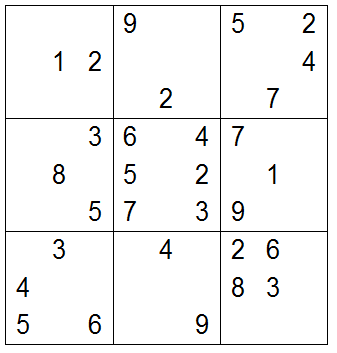
\includegraphics[scale=0.5]{images/ASTARExample/ini.PNG}
	\end{minipage} \hfill
	\begin{minipage}{.45\textwidth}
	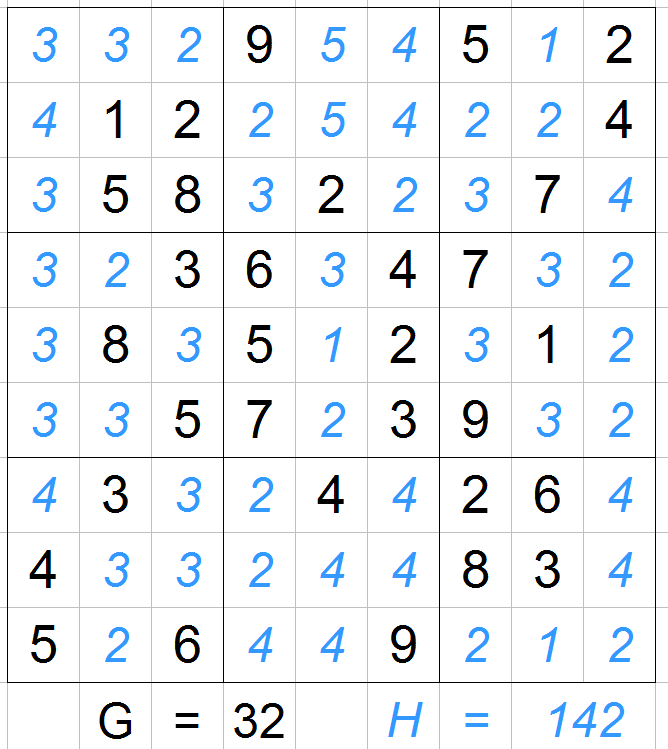
\includegraphics[scale=0.3]{images/ASTARExample/ini_H.PNG}
	\end{minipage}
}

	\pause[2]

\only<2>{
	\begin{minipage}{.45\textwidth}
	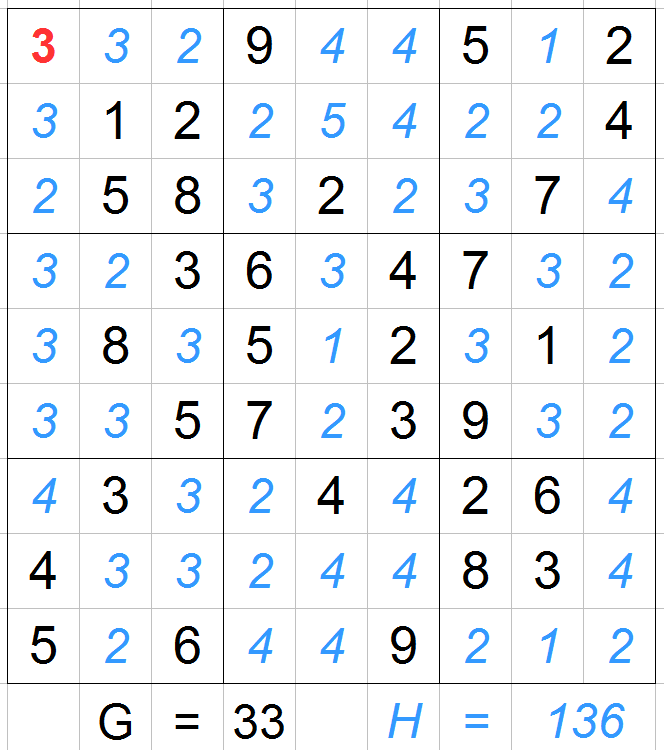
\includegraphics[scale=0.15]{images/ASTARExample/1_1.PNG}
	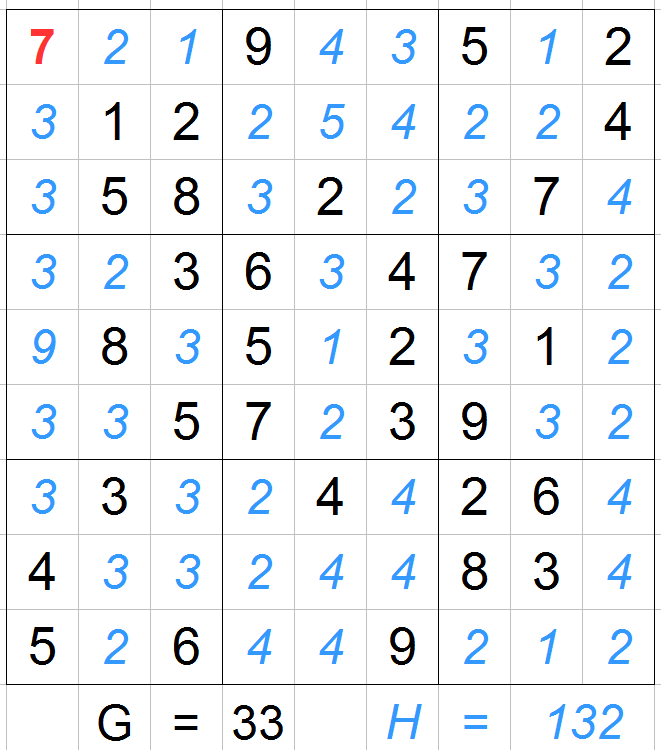
\includegraphics[scale=0.15]{images/ASTARExample/1_3.PNG}
	\end{minipage}\hfill
	\begin{minipage}{.45\textwidth}
	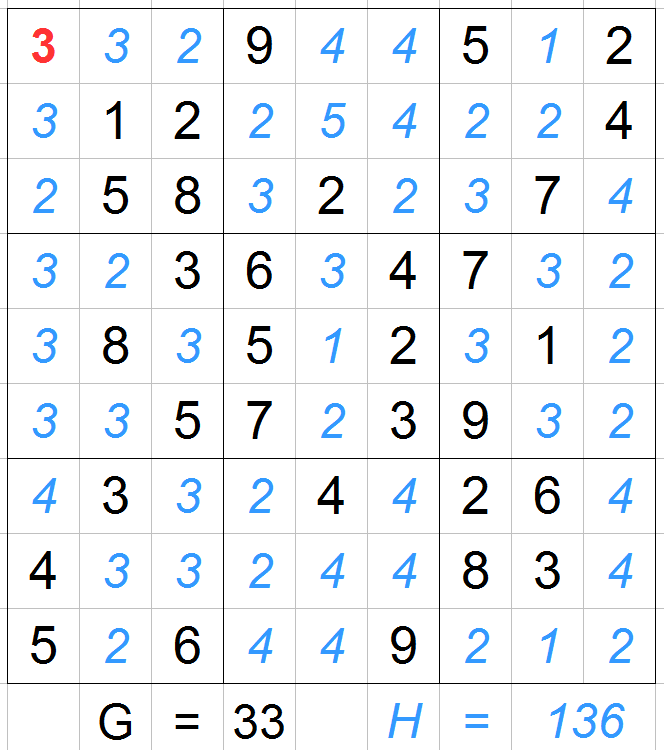
\includegraphics[scale=0.15]{images/ASTARExample/1_1.PNG}
	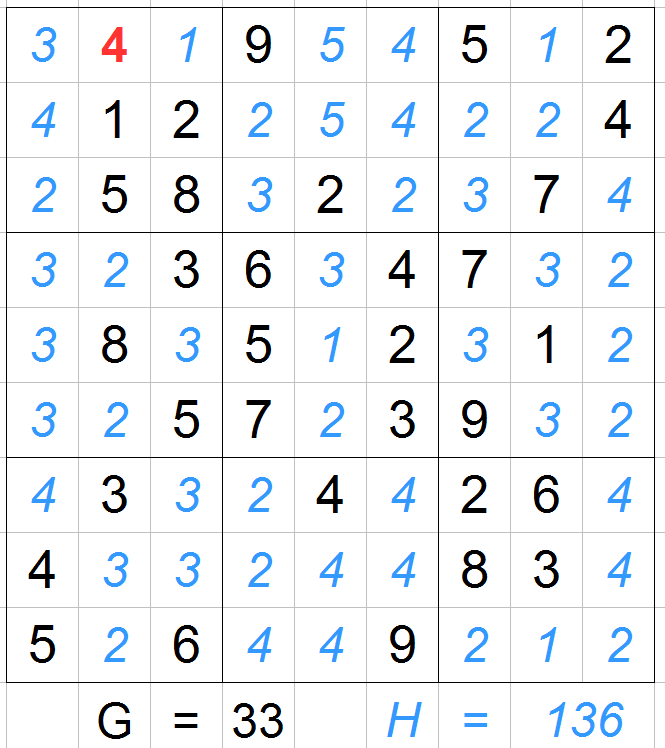
\includegraphics[scale=0.15]{images/ASTARExample/1_4.PNG}
	\end{minipage}
}

	\pause[3]

\only<3>{
	\begin{minipage}{.2\textwidth}
	\huge{...}
	\end{minipage}\hfill
	\begin{minipage}{.8\textwidth}
	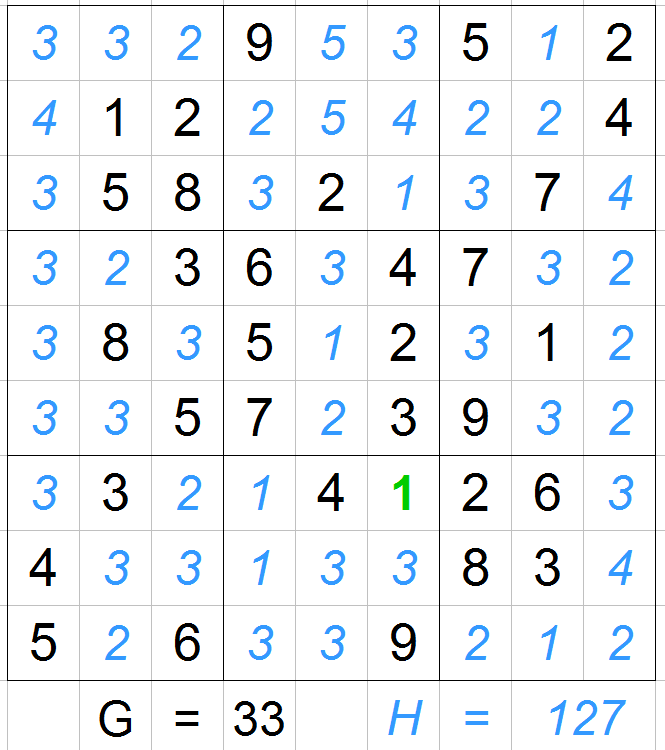
\includegraphics[scale=0.3]{images/ASTARExample/1.PNG}
	\end{minipage}
}

	\pause[4]

\only<4>{
	\begin{minipage}{.45\textwidth}
	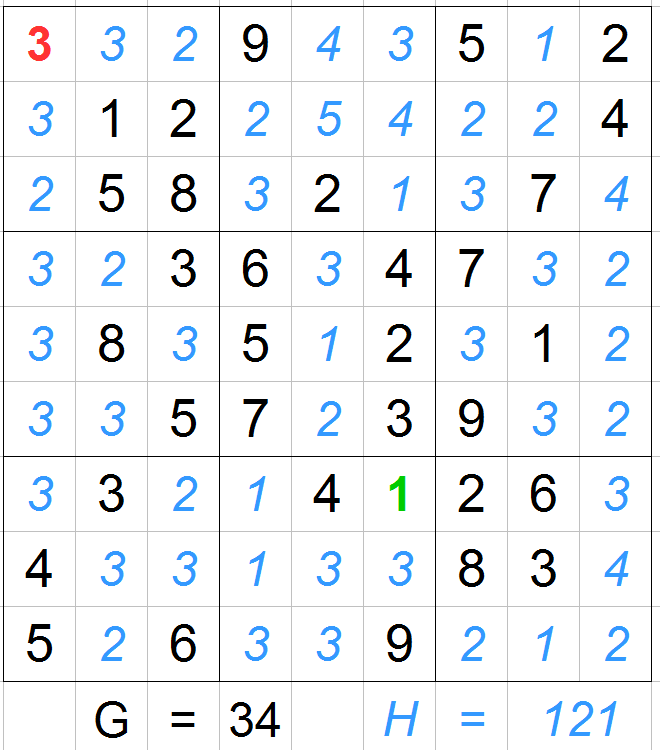
\includegraphics[scale=0.15]{images/ASTARExample/2_1.PNG}

	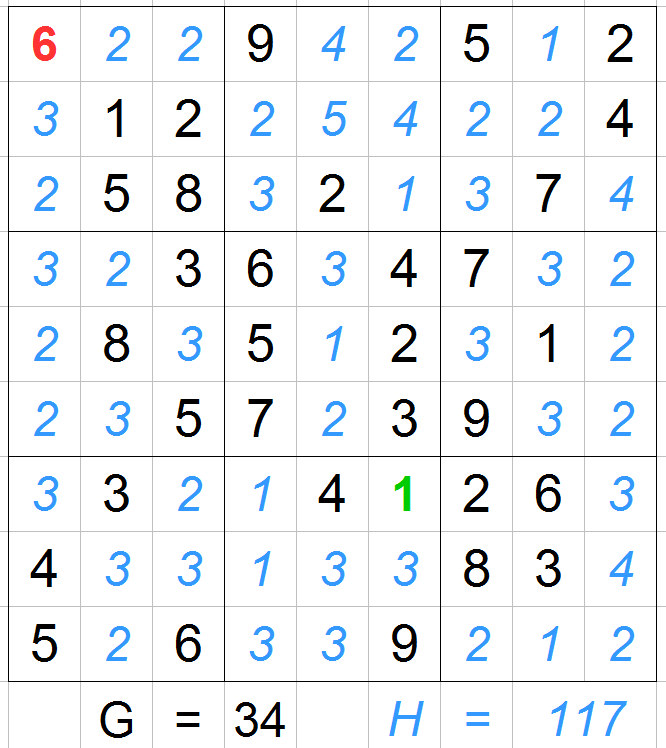
\includegraphics[scale=0.15]{images/ASTARExample/2_2.PNG}
	\end{minipage}\hfill
	\begin{minipage}{.05\textwidth}
	\huge{...}
	\end{minipage}\hfill
	\begin{minipage}{.45\textwidth}
	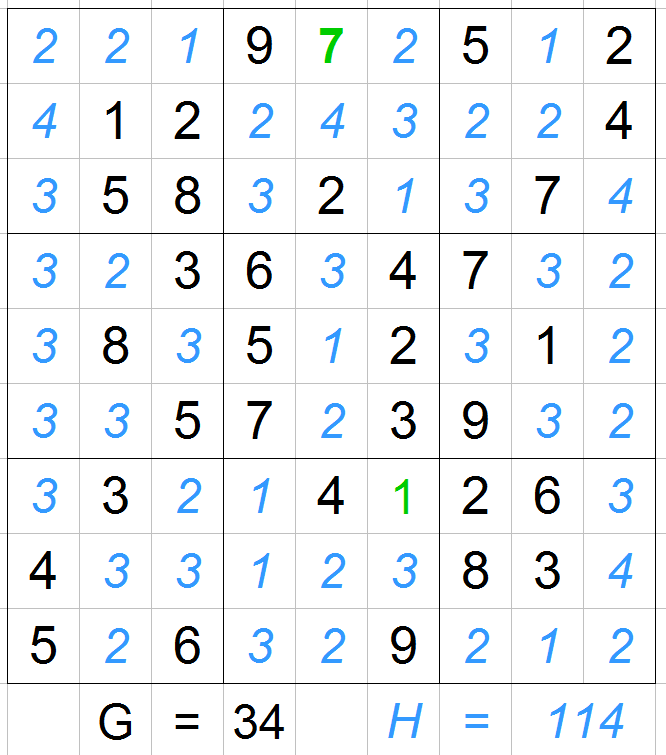
\includegraphics[scale=0.2]{images/ASTARExample/2.PNG}
	\end{minipage}
}
\end{frame}


    \section{Modélisation}
        \subsection{Algorithme génétique}
            
\begin{frame}
    \frametitle{Diagramme de classes}
    \begin{block}{Diagramme de classes}
        \begin{center}
            \includegraphics[scale=0.4]{diagrams/AGenClass.png}
        \end{center}
    \end{block}
\end{frame}

        \subsection{Éco-résolution}
            
\begin{frame}
    \frametitle{Éco-résolution}
    
    		\begin{block}{Diagramme de Classe}
    		\begin{center}
     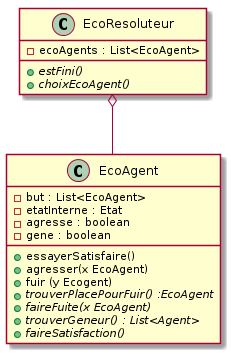
\includegraphics[scale=0.4]{diagrams/ClasseEcoResolution1.png}
    \end{center}
    		    

    		\end{block}

\end{frame}

\begin{frame}
    \frametitle{Éco-résolution}
    		\begin{block}{Diagramme de Classe}
    		\begin{center}
    		
    		     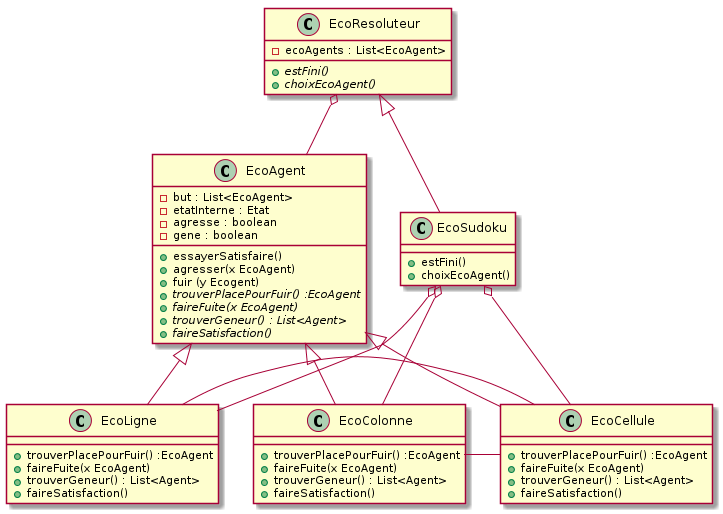
\includegraphics[scale=0.3]{diagrams/ClasseEcoResolution2.png}
    		\end{center}

    		\end{block}

\end{frame}

\begin{frame}
    \frametitle{Éco-résolution}
    		\begin{block}{Diagramme de Séquence}
    		    		\begin{center}

    		     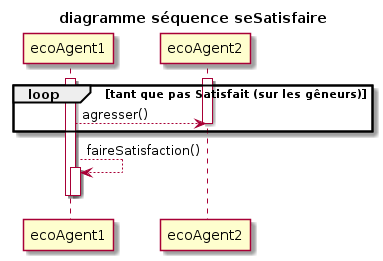
\includegraphics[scale=0.4]{diagrams/sequenceEcoResolution1.png}
    		\end{center}

    		\end{block}

\end{frame}

\begin{frame}
    \frametitle{Éco-résolution}
    		\begin{block}{Diagramme de Séquence}
    		    		\begin{center}

    		     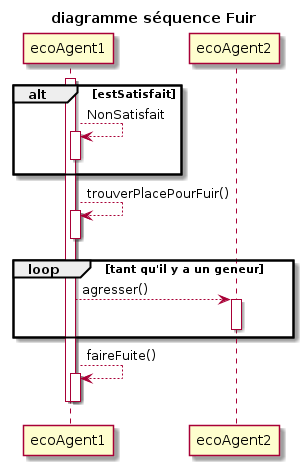
\includegraphics[scale=0.4]{diagrams/sequenceEcoResolution2.png}
    		\end{center}

    		\end{block}

\end{frame}

        \subsection{A*}
            
\begin{frame}
    \frametitle{A*}
\end{frame}

    \section{Résultats/démonstration}
        \subsection{Algorithme génétique}
            
\begin{frame}
    \frametitle{Algorithme génétique}
\end{frame}

        \subsection{Éco-résolution}
            
\begin{frame}
    \frametitle{Éco-résolution}
\end{frame}

        \subsection{A*}
            
\begin{frame}
    \frametitle{A*}
\end{frame}

    \section{Conclusion}
        \subsection{}
            \chapter{Conclusion}
   
Nous avons pu voir que l'algorithme $A^{*}$, la programmation génétique et l'éco-résolution s'appliquait à notre problème de résolution du sudoku. \\
Mais il n'y a bien évidemment pas que ces trois méthodes qui auraient pu nous permettre de résoudre le sudoku. \\
En effet, nous aurions pu voir ce problème comme étant un problème de coloration de graphe. Chaque case étant un nœud du graphe et étant reliée à toutes les cases de sa ligne, de sa colonne et son bloc. Chaque couleur aurait représenté un numéro. \\
Nous aurions également pu voir la résolution de sudoku comme étant un problème de planification 

Enfin, il est évident que la résolution du sudoku par la programmation par contrainte est la résolution la plus facile à coder et la plus efficace.
\end{document}
